\documentclass[dvipdfmx]{jsarticle}
\setcounter{section}{2}
\setcounter{subsection}{2}
\usepackage{xr}
\externaldocument{2.2.1}
\externaldocument{2.1.2}
\externaldocument{2.2.2}
\usepackage{amsmath,amsfonts,amssymb,array,comment,mathtools,url,docmute}
\usepackage{longtable,booktabs,dcolumn,tabularx,mathtools,multirow,colortbl,xcolor}
\usepackage[dvipdfmx]{graphics}
\usepackage{bmpsize}
\usepackage{amsthm}
\usepackage{enumitem}
\setlistdepth{20}
\renewlist{itemize}{itemize}{20}
\setlist[itemize]{label=•}
\renewlist{enumerate}{enumerate}{20}
\setlist[enumerate]{label=\arabic*.}
\setcounter{MaxMatrixCols}{20}
\setcounter{tocdepth}{3}
\newcommand{\rotin}{\text{\rotatebox[origin=c]{90}{$\in $}}}
\newcommand{\amap}[6]{\text{\raisebox{-0.7cm}{\begin{tikzpicture} 
  \node (a) at (0, 1) {$\textstyle{#2}$};
  \node (b) at (#6, 1) {$\textstyle{#3}$};
  \node (c) at (0, 0) {$\textstyle{#4}$};
  \node (d) at (#6, 0) {$\textstyle{#5}$};
  \node (x) at (0, 0.5) {$\rotin $};
  \node (x) at (#6, 0.5) {$\rotin $};
  \draw[->] (a) to node[xshift=0pt, yshift=7pt] {$\textstyle{\scriptstyle{#1}}$} (b);
  \draw[|->] (c) to node[xshift=0pt, yshift=7pt] {$\textstyle{\scriptstyle{#1}}$} (d);
\end{tikzpicture}}}}
\newcommand{\twomaps}[9]{\text{\raisebox{-0.7cm}{\begin{tikzpicture} 
  \node (a) at (0, 1) {$\textstyle{#3}$};
  \node (b) at (#9, 1) {$\textstyle{#4}$};
  \node (c) at (#9+#9, 1) {$\textstyle{#5}$};
  \node (d) at (0, 0) {$\textstyle{#6}$};
  \node (e) at (#9, 0) {$\textstyle{#7}$};
  \node (f) at (#9+#9, 0) {$\textstyle{#8}$};
  \node (x) at (0, 0.5) {$\rotin $};
  \node (x) at (#9, 0.5) {$\rotin $};
  \node (x) at (#9+#9, 0.5) {$\rotin $};
  \draw[->] (a) to node[xshift=0pt, yshift=7pt] {$\textstyle{\scriptstyle{#1}}$} (b);
  \draw[|->] (d) to node[xshift=0pt, yshift=7pt] {$\textstyle{\scriptstyle{#2}}$} (e);
  \draw[->] (b) to node[xshift=0pt, yshift=7pt] {$\textstyle{\scriptstyle{#1}}$} (c);
  \draw[|->] (e) to node[xshift=0pt, yshift=7pt] {$\textstyle{\scriptstyle{#2}}$} (f);
\end{tikzpicture}}}}
\renewcommand{\thesection}{第\arabic{section}部}
\renewcommand{\thesubsection}{\arabic{section}.\arabic{subsection}}
\renewcommand{\thesubsubsection}{\arabic{section}.\arabic{subsection}.\arabic{subsubsection}}
\everymath{\displaystyle}
\allowdisplaybreaks[4]
\usepackage{vtable}
\theoremstyle{definition}
\newtheorem{thm}{定理}[subsection]
\newtheorem*{thm*}{定理}
\newtheorem{dfn}{定義}[subsection]
\newtheorem*{dfn*}{定義}
\newtheorem{axs}[dfn]{公理}
\newtheorem*{axs*}{公理}
\renewcommand{\headfont}{\bfseries}
\makeatletter
  \renewcommand{\section}{%
    \@startsection{section}{1}{\z@}%
    {\Cvs}{\Cvs}%
    {\normalfont\huge\headfont\raggedright}}
\makeatother
\makeatletter
  \renewcommand{\subsection}{%
    \@startsection{subsection}{2}{\z@}%
    {0.5\Cvs}{0.5\Cvs}%
    {\normalfont\LARGE\headfont\raggedright}}
\makeatother
\makeatletter
  \renewcommand{\subsubsection}{%
    \@startsection{subsubsection}{3}{\z@}%
    {0.4\Cvs}{0.4\Cvs}%
    {\normalfont\Large\headfont\raggedright}}
\makeatother
\makeatletter
\renewenvironment{proof}[1][\proofname]{\par
  \pushQED{\qed}%
  \normalfont \topsep6\p@\@plus6\p@\relax
  \trivlist
  \item\relax
  {
  #1\@addpunct{.}}\hspace\labelsep\ignorespaces
}{%
  \popQED\endtrivlist\@endpefalse
}
\makeatother
\renewcommand{\proofname}{\textbf{証明}}
\usepackage{tikz,graphics}
\usepackage[dvipdfmx]{hyperref}
\usepackage{pxjahyper}
\hypersetup{
 setpagesize=false,
 bookmarks=true,
 bookmarksdepth=tocdepth,
 bookmarksnumbered=true,
 colorlinks=false,
 pdftitle={},
 pdfsubject={},
 pdfauthor={},
 pdfkeywords={}}
\begin{document}
%\hypertarget{hamilton-cayleyux306eux5b9aux7406}{%
\subsection{Hamilton-Cayleyの定理}%\label{hamilton-cayleyux306eux5b9aux7406}}
%\hypertarget{ux884cux5217ux306eux4e09ux89d2ux5316}{%
\subsubsection{行列の三角化}%\label{ux884cux5217ux306eux4e09ux89d2ux5316}}
\begin{thm}\label{2.2.3.1}
代数的閉体$K$上の$n$次元vector空間$V$が与えられたとき、$f:V \rightarrow V$なる任意の線形写像$f$の固有多項式$\varPhi_{f}$はあるその体$K$の元々$\lambda_{i}$を用いて次式のように変形されることができる。
\begin{align*}
\varPhi_{f} = \prod_{i \in \varLambda_{n}} \left( X - \lambda_{i} \right)
\end{align*}
\end{thm}
その証明は残念ながら代数学の多項式環の知識をかなり要求するので、多項式環の書籍にゆずることにする。
\begin{thm}[代数学の基本定理]\label{2.2.3.2}
体$\mathbb{C}$上の$n$次元vector空間$V$が与えられたとき、$f:V \rightarrow V$なる任意の線形写像$f$の固有多項式$\varPhi_{f}$の任意の複素数$z$による像$\varPhi_{f}(z)$がある複素数たち$\lambda_{i}$を用いて次式のように変形されることができる。
\begin{align*}
\varPhi_{f}(z) = \prod_{i \in \varLambda_{n}} \left( z - \lambda_{i} \right)
\end{align*}
\end{thm}
その証明は代数学の基本定理による\footnote{そんなに代数学の基本定理って感じなのかなぁ…? 代数学に複素数とか実数を持ち込むのもなんだかなぁ…。}。
\begin{thm}[三角化定理]\label{2.2.3.3}
代数的閉体$K$上の$n$次元vector空間$V$、線型写像$f:V \rightarrow V$、これの$n$つの固有値たち$\lambda_{i}$が与えられたとき、ある基底$\mathcal{B}$が存在してその線形写像$f$のその基底$\mathcal{B}$に関する表現行列$[ f]_{\mathcal{B}}^{\mathcal{B}}$は次式のように上三角行列で表されることができる。
\begin{align*}
[ f]_{\mathcal{B}}^{\mathcal{B}} = \begin{pmatrix}
\lambda_{1} & \  & \  & * \\
\  & \lambda_{2} & \  & \  \\
\  & \  & \ddots & \  \\
O & \  & \  & \lambda_{n} \\
\end{pmatrix}
\end{align*}\par
同様にして、ある基底$\mathcal{C}$が存在してその線形写像$f$のその基底$\mathcal{C}$に関する表現行列$[ f]_{\mathcal{C}}^{\mathcal{C}}$は次式のように下三角行列で表されることができる。
\begin{align*}
[ f]_{\mathcal{C}}^{\mathcal{C}} = \begin{pmatrix}
\lambda_{1} & \  & \  & O \\
\  & \lambda_{2} & \  & \  \\
\  & \  & \ddots & \  \\
* & \  & \  & \lambda_{n} \\
\end{pmatrix}
\end{align*}
この定理を三角化定理という。
\end{thm}\par
ここでは、上の主張どちらも同様にして示されるので、下三角行列の場合のみ証明を与えることにしておこう。
\begin{proof}
代数的閉体$K$上の$n$次元vector空間$V$、線型写像$f:V \rightarrow V$、これの$n$つの固有値たち$\lambda_{i}$が与えられたとする。$n = 1$のときでは明らかであるから、$n = k$のとき、ある基底が存在してその線形写像$f$のその基底に関する表現行列が上三角行列で表されることができると仮定しよう。$n = k + 1$のとき、その体$K$は代数的閉体なので、これの1つの固有vector$\mathbf{v}_{k + 1}$を含むvectorsの組$\left\langle \mathbf{v}_{i} \right\rangle_{i \in \varLambda_{k + 1}}$がそのvector空間$V$の基底となるようにとられるとする。$\lambda_{*} = \lambda_{k + 1}$、$\mathbf{v}_{*} = \mathbf{v}_{k + 1}$、$W = \mathrm{span}\left\{ \mathbf{v}_{i} \right\}_{i \in \varLambda_{k}}$として定理\ref{2.2.1.6}より次のようになるかつ、
\begin{align*}
V = W \oplus \mathrm{span}\left\{ \mathbf{v}_{*} \right\}
\end{align*}
$\forall\mathbf{v} \in W$に対し、$f\left( \mathbf{v} \right) \in V$が成り立つので、次式のようなその体$K$の元$c$とvector$\widetilde{\mathbf{v}}$が一意的に存在する。
\begin{align*}
f\left( \mathbf{v} \right) = \widetilde{\mathbf{v}} \oplus c\mathbf{v}_{*}
\end{align*}\par
また、その集合$W$はその代数的閉体$K$上のそのvector空間$V$の部分空間である。これにより、次式のような写像$f_{*}$が定義されると、
\begin{align*}
f_{*}:W \rightarrow W;\mathbf{v} \mapsto \widetilde{\mathbf{v}}
\end{align*}
$f_{*}\left( \mathbf{v} \right) = f\left( \mathbf{v} \right) - c\mathbf{v}_{*}$が成り立つ。ここで、$\forall k,l \in K\forall\mathbf{v},\mathbf{w} \in W$に対し、次のようにおくと、
\begin{align*}
f_{*}\left( \mathbf{v} \right) = f\left( \mathbf{v} \right) - c\mathbf{v}_{*},\ \ f_{*}\left( \mathbf{w} \right) = f\left( \mathbf{w} \right) - d\mathbf{v}_{*}
\end{align*}
次のようになり、
\begin{align*}
f_{*}\left( k\mathbf{v} + l\mathbf{w} \right) &= f\left( k\mathbf{v} + l\mathbf{w} \right) - C\mathbf{v}_{*}\\
&= kf\left( \mathbf{v} \right) + lf\left( \mathbf{w} \right) - C\mathbf{v}_{*}\\
&= k\left( c\mathbf{v}_{*} + f_{*}\left( \mathbf{v} \right) \right) + l\left( d\mathbf{v}_{*} + f_{*}\left( \mathbf{w} \right) \right) - C\mathbf{v}_{*}\\
&= kc\mathbf{v}_{*} + kf_{*}\left( \mathbf{v} \right) + ld\mathbf{v}_{1} + lf_{*}\left( \mathbf{w} \right) - C\mathbf{v}_{*}\\
&= kf_{*}\left( \mathbf{v} \right) + lf_{*}\left( \mathbf{w} \right) + (kc + ld - C)\mathbf{v}_{*}\\
&= \left( kf_{*}\left( \mathbf{v} \right) + lf_{*}\left( \mathbf{w} \right) \right) \oplus (kc + ld - C)\mathbf{v}_{*}
\end{align*}
次式が成り立つので、
\begin{align*}
f_{*}\left( k\mathbf{v} + l\mathbf{w} \right),kf_{*}\left( \mathbf{v} \right) + lf_{*}\left( \mathbf{w} \right) \in W,\ \ (kc + ld - C)\mathbf{v}_{*} \in \mathrm{span}\left\{ \mathbf{v}_{*} \right\}
\end{align*}
$kc + ld - C = 0$が成り立つことになる。したがって、次のようになる。
\begin{align*}
f_{*}\left( k\mathbf{v} + l\mathbf{w} \right) = kf_{*}\left( \mathbf{v} \right) + lf_{*}\left( \mathbf{w} \right)
\end{align*}
これにより、その写像$f_{*}$は線形的であることが分かった。\par
ここで、その基底$\left\langle \mathbf{v}_{i} \right\rangle_{i \in \varLambda_{k + 1}}$を$\mathcal{C}$、その基底$\left\langle \mathbf{v}_{i} \right\rangle_{i \in \varLambda_{k}}$を$\mathcal{C}_{*}$とおかれると、これらに関するそれらの線形写像たち$f$、$f_{*}$の表現行列たち$[ f]_{\mathcal{C}}^{\mathcal{C}}$、$\left[ f_{*} \right]_{\mathcal{C}_{*}}^{\mathcal{C}_{*}}$を用いて考えられれば、固有vectorの定義より$f\left( \mathbf{v}_{*} \right) = \lambda_{*}\mathbf{v}_{*}$が成り立ち、そのvector空間$K^{k + 1}$の標準直交基底を$\left\langle \mathbf{e}_{i} \right\rangle_{i \in \varLambda_{k + 1}}$とおけば、その基底$\mathcal{C}$に関する基底変換における線形同型写像$\varphi_{\mathcal{C}}$を用いて$\mathbf{e}_{*} = \mathbf{e}_{k + 1}$として$\varphi_{\mathcal{C}}\left( \mathbf{v}_{*} \right) = \mathbf{e}_{*}$が成り立つかつ、次式が成り立つことから、
\begin{center}
  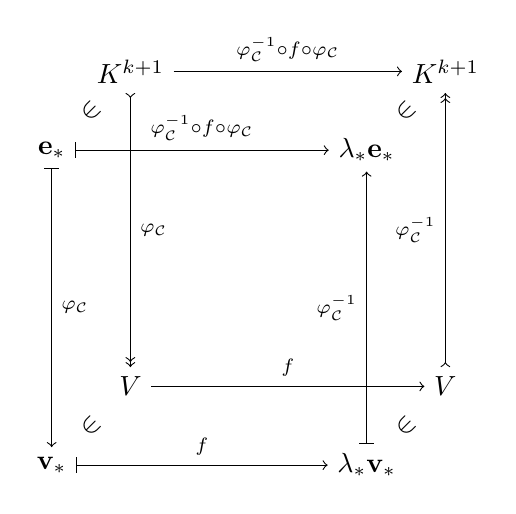
\begin{tikzpicture}[auto]

    \node (a) at (1, 1) {$V$};
    \node (b) at (5, 1) {$V$};
    \node (c) at (1, 5) {$K^{k+1} $};
    \node (d) at (5, 5) {$K^{k+1} $};
    \node (e) at (0, 4) {${\bf e}_* $};
    \node (f) at (4, 4) {$\lambda_* {\bf e}_* $};
    \node (g) at (0.5, 4.5) {\rotatebox{45}{$\in $} };
    \node (h) at (4.5, 4.5) {\rotatebox{45}{$\in $} };
    \node (i) at (0, 0) {${\bf v}_* $};
    \node (j) at (4, 0) {$\lambda_* {\bf v}_* $};
    \node (k) at (0.5, 0.5) {\rotatebox{45}{$\in $} };
    \node (l) at (4.5, 0.5) {\rotatebox{45}{$\in $} };
    
    \draw [->] (c) to node {$\scriptstyle \varphi_{\mathcal C}^{-1} \circ f \circ \varphi_{\mathcal C} $} (d);
    \draw [|->] (e) to node {$\scriptstyle \varphi_{\mathcal C}^{-1} \circ f \circ \varphi_{\mathcal C} $} (f);
    \draw [>->>] (c) to node {$\scriptstyle \varphi_{\mathcal C} $} (a);
    \draw [|->] (e) to node {$\scriptstyle \varphi_{\mathcal C} $} (i);
    \draw [->] (a) to node {$\scriptstyle f$} (b);
    \draw [|->] (i) to node {$\scriptstyle f$} (j);
    \draw [>->>] (b) to node {$\scriptstyle \varphi_{\mathcal C}^{-1} $} (d);
    \draw [|->] (j) to node {$\scriptstyle \varphi_{\mathcal C}^{-1} $} (f);

\end{tikzpicture}
\end{center}
その表現行列$[ f]_{\mathcal{C}}^{\mathcal{C}}$の第$k + 1$列は$\begin{pmatrix}
O \\
\lambda_{*} \\
\end{pmatrix}$という形になることが分かる。さらに、$\forall\mathbf{v} \oplus l_{*}\mathbf{v}_{*} \in V = W \oplus \mathrm{span}\left\{ \mathbf{v}_{*} \right\}$に対し、$\mathbf{v} = \sum_{i \in \varLambda_{k}} {l_{i}\mathbf{v}_{i}}$、$f_{*}\left( \mathbf{v} \right) = \sum_{i \in \varLambda_{k}} {\widetilde{l_{i}}\mathbf{v}_{i}}$、$\mathbf{l} = \begin{pmatrix}
l_{1} \\
 \vdots \\
l_{k} \\
\end{pmatrix}$、$\widetilde{\mathbf{l}} = \begin{pmatrix}
\widetilde{l_{1}} \\
 \vdots \\
\widetilde{l_{k + 1}} \\
c \\
\end{pmatrix}$とすると、次式のようになることから、
\begin{center}
  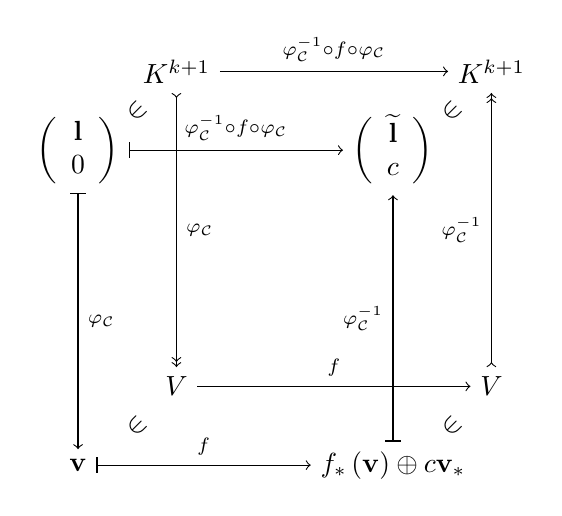
\begin{tikzpicture}[auto]
    \node (a) at (1, 1) {$V$};
    \node (b) at (5, 1) {$V$};
    \node (c) at (1, 5) {$K^{k+1} $};
    \node (d) at (5, 5) {$K^{k+1} $};
    \node (e) at (-0.25, 4) {$\left( \begin{array}{c} {\bf l} \\ 0 \end{array} \right) $};
    \node (f) at (3.75, 4) {$\left( \begin{array}{c} \widetilde{{\bf l} } \\ c \end{array} \right) $};
    \node (g) at (0.5, 4.5) {\rotatebox{45}{$\in $} };
    \node (h) at (4.5, 4.5) {\rotatebox{45}{$\in $} };
    \node (i) at (-0.25, 0) {${\bf v} $};
    \node (j) at (3.75, 0) {$f_* \left( {\bf v} \right) \oplus c{\bf v}_* $};
    \node (k) at (0.5, 0.5) {\rotatebox{45}{$\in $} };
    \node (l) at (4.5, 0.5) {\rotatebox{45}{$\in $} };
    
    \draw [->] (c) to node {$\scriptstyle \varphi_{\mathcal C}^{-1} \circ f \circ \varphi_{\mathcal C} $} (d);
    \draw [|->] (e) to node {$\scriptstyle \varphi_{\mathcal C}^{-1} \circ f \circ \varphi_{\mathcal C} $} (f);
    \draw [>->>] (c) to node {$\scriptstyle \varphi_{\mathcal C} $} (a);
    \draw [|->] (e) to node {$\scriptstyle \varphi_{\mathcal C} $} (i);
    \draw [->] (a) to node {$\scriptstyle f$} (b);
    \draw [|->] (i) to node {$\scriptstyle f$} (j);
    \draw [>->>] (b) to node {$\scriptstyle \varphi_{\mathcal C}^{-1} $} (d);
    \draw [|->] (j) to node {$\scriptstyle \varphi_{\mathcal C}^{-1} $} (f);
    
\end{tikzpicture}
\end{center}
次のようになる。
\begin{align*}
[ f]_{\mathcal{C}}^{\mathcal{C}}\begin{pmatrix}
\mathbf{l} \\
l_{*} \\
\end{pmatrix} &= [ f]_{\mathcal{C}}^{\mathcal{C}}\begin{pmatrix}
\mathbf{l} \\
0 \\
\end{pmatrix} + [ f]_{\mathcal{C}}^{\mathcal{C}}\begin{pmatrix}
\mathbf{0} \\
l_{*} \\
\end{pmatrix}\\
&= \begin{pmatrix}
\widetilde{\mathbf{l}} \\
c \\
\end{pmatrix} + \begin{pmatrix}
* & O \\
* & \lambda_{*} \\
\end{pmatrix}\begin{pmatrix}
\mathbf{0} \\
l_{*} \\
\end{pmatrix}\\
&= \begin{pmatrix}
\left[ f_{*} \right]_{\mathcal{C}_{*}}^{\mathcal{C}_{*}}\mathbf{l} \\
c \\
\end{pmatrix} + \begin{pmatrix}
\mathbf{0} \\
\lambda_{*}l_{*} \\
\end{pmatrix}\\
&= \begin{pmatrix}
\left[ f_{*} \right]_{\mathcal{C}_{*}}^{\mathcal{C}_{*}}\mathbf{l} \\
c + \lambda_{*}l_{*} \\
\end{pmatrix}\\
&= \begin{pmatrix}
\left[ f_{*} \right]_{\mathcal{C}_{*}}^{\mathcal{C}_{*}} & O \\
* & \lambda_{*} \\
\end{pmatrix}\begin{pmatrix}
\mathbf{l} \\
l_{*} \\
\end{pmatrix}
\end{align*}
したがって、$[ f]_{\mathcal{C}}^{\mathcal{C}} = \begin{pmatrix}
\left[ f_{*} \right]_{\mathcal{C}_{*}}^{\mathcal{C}_{*}} & O \\
* & \lambda_{*} \\
\end{pmatrix}$が成り立つ。ここで、仮定より予め基底$\mathcal{C}_{*}$を上手く選んでおけば、その線形写像$f_{*}$のその基底$\mathcal{C}_{*}$に関する表現行列$\left[ f_{*} \right]_{\mathcal{C}_{*}}^{\mathcal{C}_{*}}$は次式のように下三角行列で表されることができるので、
\begin{align*}
\left[ f_{*} \right]_{\mathcal{C}_{*}}^{\mathcal{C}_{*}} = \begin{pmatrix}
\lambda_{1} & \  & O \\
\  & \ddots & \  \\
* & \  & \lambda_{k} \\
\end{pmatrix}
\end{align*}
次式が得られる。
\begin{align*}
[ f]_{\mathcal{C}}^{\mathcal{C}} &= \begin{pmatrix}
\begin{pmatrix}
\lambda_{1} & \  & O \\
\  & \ddots & \  \\
* & \  & \lambda_{k} \\
\end{pmatrix} & O \\
* & \lambda_{k + 1} \\
\end{pmatrix}\\
&= \begin{pmatrix}
\lambda_{1} & \  & \  & O \\
\  & \lambda_{2} & \  & \  \\
\  & \  & \ddots & \  \\
* & \  & \  & \lambda_{k + 1} \\
\end{pmatrix}
\end{align*}
\end{proof}
%\hypertarget{frobeniusux306eux5b9aux7406}{%
\subsubsection{Frobeniusの定理}%\label{frobeniusux306eux5b9aux7406}}
\begin{dfn}
体$K$上の$n$次元vector空間$V$、多項式環$K[ X]$の$\rho = \sum_{i \in \varLambda_{r} \cup \left\{ 0 \right\}} {k_{i}X^{i}}$なる多項式$\rho$が与えられたとき、$f:V \rightarrow V$なる線形写像$f$を用いて、線形写像$f^{0}$、合成$\circ$をそれぞれ恒等写像$I_{V}$、積とみなすことにすると、次式のような写像$\rho(f)$をその多項式$\rho$の変数$X$にその線形写像$f$を代入した写像という。
\begin{align*}
\rho(f) = \sum_{i \in \varLambda_{r} \cup \left\{ 0 \right\}} {k_{i}f^{i}} = k_{0}I_{V} + k_{1}f + k_{2}f \circ f + \cdots + k_{r}{\underbrace{f \circ \cdots \circ f}_{r\ \mathrm{times}}}:V \rightarrow V
\end{align*}
\end{dfn}
\begin{thm}\label{2.2.3.4}
体$K$上の$n$次元vector空間$V$が与えられたとき、多項式環$K[ X]$の多項式$\rho$の変数$X$に線形写像$f:V \rightarrow V$を代入した写像$\rho(f)$も線形的である。
\end{thm}
\begin{proof}
体$K$上の$n$次元vector空間$V$が与えられたとき、多項式環$K[ X]$の$\rho = \sum_{i \in \varLambda_{r} \cup \left\{ 0 \right\}} {k_{i}X^{i}}$なる多項式$\rho$の変数$X$に線形写像$f:V \rightarrow V$を代入した写像$\rho(f)$において、$\forall k,l \in K\forall\mathbf{v},\mathbf{w} \in V$に対し、次のようになる。
\begin{align*}
\rho(f)\left( k\mathbf{v} + l\mathbf{w} \right) &= \left( \sum_{i \in \varLambda_{r} \cup \left\{ 0 \right\}} {k_{i}f^{i}} \right)\left( k\mathbf{v} + l\mathbf{w} \right)\\
&= \sum_{i \in \varLambda_{r} \cup \left\{ 0 \right\}} {k_{i}f^{i}\left( k\mathbf{v} + l\mathbf{w} \right)}\\
&= \sum_{i \in \varLambda_{r} \cup \left\{ 0 \right\}} {k_{i}\left( kf^{i}\left( \mathbf{v} \right) + lf^{i}\left( \mathbf{w} \right) \right)}\\
&= \sum_{i \in \varLambda_{r} \cup \left\{ 0 \right\}} \left( k_{i}kf^{i}\left( \mathbf{v} \right) + k_{i}lf^{i}\left( \mathbf{w} \right) \right)\\
&= k\sum_{i \in \varLambda_{r} \cup \left\{ 0 \right\}} {k_{i}f^{i}\left( \mathbf{v} \right)} + l\sum_{i \in \varLambda_{r} \cup \left\{ 0 \right\}} {k_{i}f^{i}\left( \mathbf{w} \right)}\\
&= k\left( \sum_{i \in \varLambda_{r} \cup \left\{ 0 \right\}} {k_{i}f^{i}} \right)\left( \mathbf{v} \right) + l\left( \sum_{i \in \varLambda_{r} \cup \left\{ 0 \right\}} {k_{i}f^{i}} \right)\left( \mathbf{w} \right)\\
&= k\rho(f)\left( \mathbf{v} \right) + l\rho(f)\left( \mathbf{w} \right)
\end{align*}
よって、その多項式$\rho$の変数$X$にその線形写像$f$を代入した写像$\rho(f)$も線形的である。
\end{proof}
\begin{thm}\label{2.2.3.5}
体$K$上の$n$次元vector空間$V$、次式のような多項式環$K[ X]$の多項式たち$\rho$、$\sigma$が与えられたとき、
\begin{align*}
\rho = \sum_{i \in \varLambda_{r} \cup \left\{ 0 \right\}} {k_{i}X^{i}},\ \ \sigma = \sum_{i \in \varLambda_{s} \cup \left\{ 0 \right\}} {l_{i}X^{i}}
\end{align*}
それらの多項式たち$\rho$、$\sigma$の変数$X$に線形写像$f:V \rightarrow V$を代入した写像たち$\rho(f)$、$\sigma(f)$について、$\sigma(f) \circ \rho(f) = \rho(f) \circ \sigma(f)$が成り立つ。
\end{thm}
\begin{proof}
体$K$上の$n$次元vector空間$V$、次式のような多項式環$K[ X]$の多項式たち$\rho$、$\sigma$が与えられたとき、
\begin{align*}
\rho = \sum_{i \in \varLambda_{r} \cup \left\{ 0 \right\}} {k_{i}X^{i}},\ \ \sigma = \sum_{i \in \varLambda_{s} \cup \left\{ 0 \right\}} {l_{i}X^{i}}
\end{align*}
それらの多項式たち$\rho$、$\sigma$の変数$X$に線形写像$f:V \rightarrow V$を代入した写像たち$\rho(f)$、$\sigma(f)$について、定理\ref{2.1.2.10}より次のようになる。
\begin{align*}
\sigma(f) \circ \rho(f) &= \left( \sum_{i \in \varLambda_{r} \cup \left\{ 0 \right\}} {k_{i}f^{i}} \right) \circ \left( \sum_{i \in \varLambda_{s} \cup \left\{ 0 \right\}} {l_{i}f^{i}} \right)\\
&= \sum_{(i,j) \in \left( \varLambda_{r} \cup \left\{ 0 \right\} \right) \times \left( \varLambda_{s} \cup \left\{ 0 \right\} \right)} {k_{i}f^{i} \circ l_{j}f^{j}}\\
&= \sum_{(i,j) \in \left( \varLambda_{r} \cup \left\{ 0 \right\} \right) \times \left( \varLambda_{s} \cup \left\{ 0 \right\} \right)} {k_{i}l_{j}f^{i + j}}\\
&= \sum_{(i,j) \in \left( \varLambda_{s} \cup \left\{ 0 \right\} \right) \times \left( \varLambda_{r} \cup \left\{ 0 \right\} \right)} {l_{i}f^{i} \circ k_{j}f^{j}}\\
&= \left( \sum_{i \in \varLambda_{s} \cup \left\{ 0 \right\}} {l_{i}f^{i}} \right) \circ \left( \sum_{i \in \varLambda_{r} \cup \left\{ 0 \right\}} {k_{i}f^{i}} \right) = \rho(f) \circ \sigma(f)
\end{align*}
\end{proof}
\begin{thm}\label{2.2.3.6}
上三角行列たち$\begin{pmatrix}
\alpha_{1} & \  & \  & * \\
\  & \alpha_{2} & \  & \  \\
\  & \  & \ddots & \  \\
O & \  & \  & \alpha_{n} \\
\end{pmatrix}$、$\begin{pmatrix}
\beta_{1} & \  & \  & * \\
\  & \beta_{2} & \  & \  \\
\  & \  & \ddots & \  \\
O & \  & \  & \beta_{n} \\
\end{pmatrix}$が与えられたとき、次式のようになる。
\begin{align*}
\begin{pmatrix}
\alpha_{1} & \  & \  & * \\
\  & \alpha_{2} & \  & \  \\
\  & \  & \ddots & \  \\
O & \  & \  & \alpha_{n} \\
\end{pmatrix}\begin{pmatrix}
\beta_{1} & \  & \  & * \\
\  & \beta_{2} & \  & \  \\
\  & \  & \ddots & \  \\
O & \  & \  & \beta_{n} \\
\end{pmatrix} = \begin{pmatrix}
\alpha_{1}\beta_{1} & \  & \  & * \\
\  & \alpha_{2}\beta_{2} & \  & \  \\
\  & \  & \ddots & \  \\
O & \  & \  & \alpha_{n}\beta_{n} \\
\end{pmatrix}
\end{align*}
同様に、下三角行列たち$\begin{pmatrix}
\alpha_{1} & \  & \  & O \\
\  & \alpha_{2} & \  & \  \\
\  & \  & \ddots & \  \\
* & \  & \  & \alpha_{n} \\
\end{pmatrix}$、$\begin{pmatrix}
\beta_{1} & \  & \  & O \\
\  & \beta_{2} & \  & \  \\
\  & \  & \ddots & \  \\
* & \  & \  & \beta_{n} \\
\end{pmatrix}$が与えられたとき、次式のようになる。
\begin{align*}
\begin{pmatrix}
\alpha_{1} & \  & \  & O \\
\  & \alpha_{2} & \  & \  \\
\  & \  & \ddots & \  \\
* & \  & \  & \alpha_{n} \\
\end{pmatrix}\begin{pmatrix}
\beta_{1} & \  & \  & O \\
\  & \beta_{2} & \  & \  \\
\  & \  & \ddots & \  \\
* & \  & \  & \beta_{n} \\
\end{pmatrix} = \begin{pmatrix}
\alpha_{1}\beta_{1} & \  & \  & O \\
\  & \alpha_{2}\beta_{2} & \  & \  \\
\  & \  & \ddots & \  \\
* & \  & \  & \alpha_{n}\beta_{n} \\
\end{pmatrix}
\end{align*}
\end{thm}
\begin{proof} $n$次正方行列でもある上三角行列たち$\begin{pmatrix}
\alpha_{1} & \  & \  & * \\
\  & \alpha_{2} & \  & \  \\
\  & \  & \ddots & \  \\
O & \  & \  & \alpha_{n} \\
\end{pmatrix}$、$\begin{pmatrix}
\beta_{1} & \  & \  & * \\
\  & \beta_{2} & \  & \  \\
\  & \  & \ddots & \  \\
O & \  & \  & \beta_{n} \\
\end{pmatrix}$が与えられたとき、これらを$\left( a_{ij} \right)_{(i,j) \in \varLambda_{n}^{2}}$、$\left( b_{ij} \right)_{(i,j) \in \varLambda_{n}^{2}}$とおくと、次のようになることから、
\begin{align*}
\sum_{k \in \varLambda_{n}} {a_{ik}b_{kj}} &= \left\{ \begin{matrix}
\sum_{k \in \varLambda_{n}} {a_{ik}b_{kj}} & \mathrm{if} & i < j \\
a_{ii}b_{ii} + \sum_{\scriptsize \begin{matrix}
k \in \varLambda_{n} \setminus \left\{ i \right\} \\
k < i \\
\end{matrix}} {a_{ik}b_{kj}} + \sum_{\scriptsize \begin{matrix}
k \in \varLambda_{n} \setminus \left\{ i \right\} \\
k > i \\
\end{matrix}} {a_{ik}b_{kj}} & \mathrm{if} & i = j \\
\sum_{\scriptsize \begin{matrix}
k \in \varLambda_{n} \\
k \leq j \\
\end{matrix}} {a_{ik}b_{kj}} + \sum_{\scriptsize \begin{matrix}
k \in \varLambda_{n} \\
j < k < i \\
\end{matrix}} {a_{ik}b_{kj}}\sum_{\scriptsize \begin{matrix}
k \in \varLambda_{n} \\
i \leq k \\
\end{matrix}} {a_{ik}b_{kj}} & \mathrm{if} & i > j \\
\end{matrix} \right.\ \\
&= \left\{ \begin{matrix}
\sum_{k \in \varLambda_{n}} {a_{ik}b_{kj}} & \mathrm{if} & i < j \\
a_{ii}b_{ii} + \sum_{\scriptsize \begin{matrix}
k \in \varLambda_{n} \setminus \left\{ i \right\} \\
k < i \\
\end{matrix}} {0b_{kj}} + \sum_{\scriptsize \begin{matrix}
k \in \varLambda_{n} \setminus \left\{ i \right\} \\
k > i \\
\end{matrix}} {a_{ik}0} & \mathrm{if} & i = j \\
\sum_{\scriptsize \begin{matrix}
k \in \varLambda_{n} \\
k \leq j \\
\end{matrix}} {0b_{kj}} + \sum_{\scriptsize \begin{matrix}
k \in \varLambda_{n} \\
j < k < i \\
\end{matrix}} 0 + \sum_{\scriptsize \begin{matrix}
k \in \varLambda_{n} \\
i \leq k \\
\end{matrix}} {a_{ik}0} & \mathrm{if} & i > j \\
\end{matrix} \right.\ \\
&= \left\{ \begin{matrix}
\sum_{k \in \varLambda_{n}} {a_{ik}b_{kj}} & \mathrm{if} & i < j \\
a_{ii}b_{ii} + 0 & \mathrm{if} & i = j \\
0 & \mathrm{if} & i > j \\
\end{matrix} \right.\ \\
&= \left\{ \begin{matrix}
\sum_{k \in \varLambda_{n}} {a_{ik}b_{kj}} & \mathrm{if} & i < j \\
\alpha_{i}\beta_{i} & \mathrm{if} & i = j \\
0 & \mathrm{if} & i > j \\
\end{matrix} \right.\ 
\end{align*}
次式のようになる。
\begin{align*}
\begin{pmatrix}
\alpha_{1} & \  & \  & * \\
\  & \alpha_{2} & \  & \  \\
\  & \  & \ddots & \  \\
O & \  & \  & \alpha_{n} \\
\end{pmatrix}\begin{pmatrix}
\beta_{1} & \  & \  & * \\
\  & \beta_{2} & \  & \  \\
\  & \  & \ddots & \  \\
O & \  & \  & \beta_{n} \\
\end{pmatrix} = \begin{pmatrix}
\alpha_{1}\beta_{1} & \  & \  & * \\
\  & \alpha_{2}\beta_{2} & \  & \  \\
\  & \  & \ddots & \  \\
O & \  & \  & \alpha_{n}\beta_{n} \\
\end{pmatrix}
\end{align*}
下三角行列についても同様にして示される。
\end{proof}
\begin{thm}[Frobeniusの定理]\label{2.2.3.7}
代数的閉体$K$上の$n$次元vector空間$V$、線型写像$f:V \rightarrow V$、これの$\forall i \in \varLambda_{n}$に対する固有値たち$\lambda_{i}$、多項式環$K[ X]$の多項式$\rho$が与えられたとき、その多項式$\rho$の変数$X$にその線形写像$f$を代入した写像$\rho(f)$の固有値たちは、$\forall i \in \varLambda_{n}$に対し、$\rho\left( \lambda_{i} \right)$と与えられる、即ち、それらの線形写像たち$f$、$\rho(f)$の固有多項式$\varPhi_{f}$、$\varPhi_{\rho(f)}$について、定理\ref{2.2.3.1}より次式のように与えられることができ、そうしたらば、
\begin{align*}
\varPhi_{f} = \prod_{i \in \varLambda_{n}} \left( X - \lambda_{i} \right)
\end{align*}
次のようになる。
\begin{align*}
\varPhi_{\rho(f)} = \prod_{i \in \varLambda_{n}} \left( X - \rho\left( \lambda_{i} \right) \right)
\end{align*}
この定理をFrobeniusの定理という。
\end{thm}
\begin{proof}
代数的閉体$K$上の$n$次元vector空間$V$、線型写像$f:V \rightarrow V$、これの$\forall i \in \varLambda_{n}$に対する固有値たち$\lambda_{i}$、$\rho = \sum_{i \in \varLambda_{r} \cup \left\{ 0 \right\}} {k_{i}X^{i}}$なる多項式環$K[ X]$の多項式$\rho$が与えられたとき、三角化定理よりある基底$\mathcal{B}$に関するその線形写像$f$の表現行列$[ f]_{\mathcal{B}}^{\mathcal{B}}$は次式のように表されることができる。
\begin{align*}
[ f]_{\mathcal{B}}^{\mathcal{B}} = \begin{pmatrix}
\lambda_{1} & \  & \  & * \\
\  & \lambda_{2} & \  & \  \\
\  & \  & \ddots & \  \\
O & \  & \  & \lambda_{n} \\
\end{pmatrix}
\end{align*}
したがって、定理\ref{2.2.3.6}より次のようになる。
\begin{align*}
\left[ \rho(f) \right]_{\mathcal{B}}^{\mathcal{B}} &= \left[ \sum_{i \in \varLambda_{r} \cup \left\{ 0 \right\}} {k_{i}f^{i}} \right]_{\mathcal{B}}^{\mathcal{B}}\\
&= \sum_{i \in \varLambda_{r} \cup \left\{ 0 \right\}} {k_{i}\left[ f^{i} \right]_{\mathcal{B}}^{\mathcal{B}}}\\
&= \sum_{i \in \varLambda_{r} \cup \left\{ 0 \right\}} {k_{i}{[ f]_{\mathcal{B}}^{\mathcal{B}}}^{i}}\\
&= \sum_{i \in \varLambda_{r} \cup \left\{ 0 \right\}} {k_{i}\begin{pmatrix}
\lambda_{1} & \  & \  & * \\
\  & \lambda_{2} & \  & \  \\
\  & \  & \ddots & \  \\
O & \  & \  & \lambda_{n} \\
\end{pmatrix}^{i}}\\
&= \sum_{i \in \varLambda_{r} \cup \left\{ 0 \right\}} {k_{i}\begin{pmatrix}
\lambda_{1}^{i} & \  & \  & * \\
\  & \lambda_{2}^{i} & \  & \  \\
\  & \  & \ddots & \  \\
O & \  & \  & \lambda_{n}^{i} \\
\end{pmatrix}}\\
&= \begin{pmatrix}
\sum_{i \in \varLambda_{r} \cup \left\{ 0 \right\}} {k_{i}\lambda_{1}^{i}} & \  & \  & * \\
\  & \sum_{i \in \varLambda_{r} \cup \left\{ 0 \right\}} {k_{i}\lambda_{2}^{i}} & \  & \  \\
\  & \  & \ddots & \  \\
O & \  & \  & \sum_{i \in \varLambda_{r} \cup \left\{ 0 \right\}} {k_{i}\lambda_{n}^{i}} \\
\end{pmatrix}\\
&= \begin{pmatrix}
\rho\left( \lambda_{1} \right) & \  & \  & * \\
\  & \rho\left( \lambda_{2} \right) & \  & \  \\
\  & \  & \ddots & \  \\
O & \  & \  & \rho\left( \lambda_{n} \right) \\
\end{pmatrix}
\end{align*}
定理\ref{2.2.2.9} 、定理\ref{2.2.3.1}より、それらの線形写像たち$f$、$\rho(f)$の固有多項式$\varPhi_{f}$、$\varPhi_{\rho(f)}$について、次式のように与えられることができ、そうしたらば、
\begin{align*}
\varPhi_{f} = \prod_{i \in \varLambda_{n}} \left( X - \lambda_{i} \right)
\end{align*}
次のようになる。
\begin{align*}
\varPhi_{\rho(f)} = \prod_{i \in \varLambda_{n}} \left( X - \rho\left( \lambda_{i} \right) \right)
\end{align*}
よって、その多項式$\rho$の変数$X$にその線形写像$f$を代入した写像$\rho(f)$の固有値たちは、$\forall i \in \varLambda_{n}$に対し、$\rho\left( \lambda_{i} \right)$と与えられる。
\end{proof}
\begin{thm}\label{2.2.3.8}
代数的閉体$K$上の$n$次元vector空間$V$、線型写像$f:V \rightarrow V$、これの固有値$\lambda$、これの固有vector$\mathbf{v}$、多項式環$K[ X]$の多項式$\rho$が与えられたとき、その多項式$\rho$の変数$X$にその線形写像$f$を代入した写像$\rho(f)$の固有値$\rho(\lambda)$の固有vectorはそのvector$\mathbf{v}$である。
\end{thm}
\begin{proof}
代数的閉体$K$上の$n$次元vector空間$V$、線型写像$f:V \rightarrow V$、これの固有値$\lambda$、これの固有vector$\mathbf{v}$、$\rho = \sum_{i \in \varLambda_{r} \cup \left\{ 0 \right\}} {k_{i}X^{i}}$なる多項式環$K[ X]$の多項式$\rho$が与えられたとき、$f\left( \mathbf{v} \right) = \lambda\mathbf{v}$が成り立つのであった。このとき、次のようになるので、
\begin{align*}
\rho(f)\left( \mathbf{v} \right) &= \left( \sum_{i \in \varLambda_{r} \cup \left\{ 0 \right\}} {k_{i}f^{i}} \right)\left( \mathbf{v} \right)\\
&= \sum_{i \in \varLambda_{r} \cup \left\{ 0 \right\}} {k_{i}f^{i}\left( \mathbf{v} \right)}\\
&= \sum_{i \in \varLambda_{r} \cup \left\{ 0 \right\}} {k_{i}\lambda^{i}\mathbf{v}}\\
&= \left( \sum_{i \in \varLambda_{r} \cup \left\{ 0 \right\}} {k_{i}\lambda^{i}} \right)\left( \mathbf{v} \right) = \rho(\lambda)\mathbf{v}
\end{align*}
その多項式$\rho$の変数$X$にその線形写像$f$を代入した写像$\rho(f)$の固有値$\rho(\lambda)$の固有vectorはそのvector$\mathbf{v}$である。
\end{proof}
%\hypertarget{hamilton-cayleyux306eux5b9aux7406-1}{%
\subsubsection{Hamilton-Cayleyの定理}%\label{hamilton-cayleyux306eux5b9aux7406-1}}
\begin{thm}[Hailiton-Cayleyの定理]\label{2.2.3.9}
代数的閉体$K$上の$n$次元vector空間$V$、線型写像$f:V \rightarrow V$、固有多項式$\varPhi_{f}$が与えられたとき、その多項式$\varPhi_{f}$の変数$X$にその線形写像$f$を代入した写像$\varPhi_{f}(f)$は零写像である、即ち、次式のようになる。
\begin{align*}
\varPhi_{f}(f):V \rightarrow V;\mathbf{v} \mapsto \mathbf{0}
\end{align*}
この定理をHailiton-Cayleyの定理という。
\end{thm}
\begin{proof}
代数的閉体$K$上の$n$次元vector空間$V$、線型写像$f:V \rightarrow V$、固有多項式$\varPhi_{f}$が与えられたとき、定理\ref{2.2.3.1}より次式のように与えられることができ、そうしたらば、
\begin{align*}
\varPhi_{f} = \prod_{i \in \varLambda_{n}} \left( X - \lambda_{i} \right)
\end{align*}
次式が成り立つ。
\begin{align*}
\varPhi_{f}(f) = \prod_{i \in \varLambda_{n}} \left( f - \lambda_{i}I_{V} \right)
\end{align*}
ここで、三角化定理よりそのvector空間$V$のある基底$\left\langle \mathbf{v}_{i} \right\rangle_{i \in \varLambda_{n}}$が存在して、これを$\mathcal{B}$とおくと、これに関するその線形写像$f$の表現行列$[ f]_{\mathcal{B}}^{\mathcal{B}}$は次式のように表されることができる。
\begin{align*}
[ f]_{\mathcal{B}}^{\mathcal{B}} = \begin{pmatrix}
\lambda_{1} & \  & \  & * \\
\  & \lambda_{2} & \  & \  \\
\  & \  & \ddots & \  \\
O & \  & \  & \lambda_{n} \\
\end{pmatrix}
\end{align*}\par
$f\left( \mathbf{v}_{1} \right) = \lambda_{1}\mathbf{v}_{1}$が成り立つので、次のようになる。
\begin{align*}
\left( f - \lambda_{1}I_{V} \right)\left( \mathbf{v}_{1} \right) &= f\left( \mathbf{v}_{1} \right) - \lambda_{1}I_{V}\left( \mathbf{v}_{1} \right)\\
&= f\left( \mathbf{v}_{1} \right) - \lambda_{1}\mathbf{v}_{1} = \mathbf{0}
\end{align*}
$m = k$のとき、$\forall m' \in \varLambda_{k}$に対し、$\prod_{i \in \varLambda_{k}} \left( f - \lambda_{i}I_{V} \right)\left( \mathbf{v}_{m'} \right) = \mathbf{0}$が成り立つと仮定しよう。$m = k + 1$のとき、$\forall i \in \varLambda_{k}$に対し、写像の合成$\circ$は、その線形写像$f$自身か恒等写像$I_{V}$に対してのみ移すので、可換的であり次のようになる。
\begin{align*}
\prod_{i \in \varLambda_{k + 1}} \left( f - \lambda_{i}I_{V} \right)\left( \mathbf{v}_{m'} \right) &= \left( f - \lambda_{k + 1}I_{V} \right) \circ \prod_{i \in \varLambda_{k}} \left( f - \lambda_{i}I_{V} \right)\left( \mathbf{v}_{m'} \right)\\
&= \left( f - \lambda_{k + 1}I_{V} \right)\left( \prod_{i \in \varLambda_{k}} \left( f - \lambda_{i}I_{V} \right)\left( \mathbf{v}_{m'} \right) \right)\\
&= \left( f - \lambda_{k + 1}I_{V} \right)\left( \mathbf{0} \right) = \mathbf{0}
\end{align*}
また、その表現行列$[ f]_{\mathcal{B}}^{\mathcal{B}}$の第$k + 1$列は$\begin{pmatrix}
* \\
\lambda_{k + 1} \\
O \\
\end{pmatrix}$と表されるので、その基底$\mathcal{B}$に関する基底変換における線形同型写像$\varphi_{\mathcal{B}}$を用いて第$k$成分のみ$1$でこれ以外の成分が$0$であるような$n$-vector$\mathbf{e}_{k}$を用いて次式のように考えられれば、
\begin{center}
  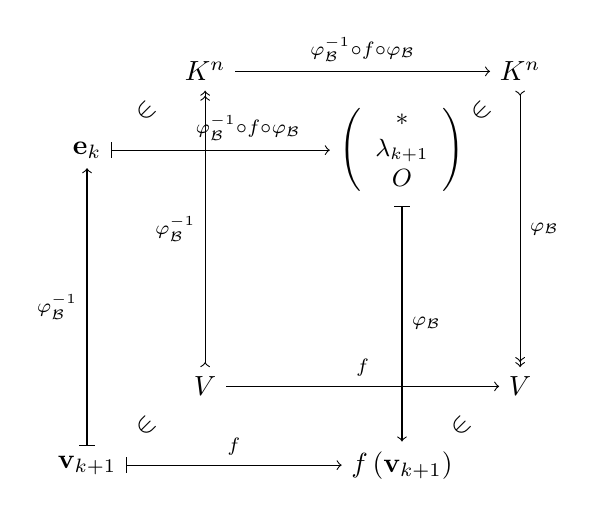
\begin{tikzpicture}[auto]

    \node (a) at (1.5, 5) {$K^n $};
    \node (b) at (5.5, 5) {$K^n $};
    \node (c) at (1.5, 1) {$V$};
    \node (d) at (5.5, 1) {$V$};
    \node (e) at (0, 4) {${\bf e}_k $};
    \node (f) at (4, 4) {${\small \left( \begin{array}{c} *\\ \lambda_{k+1} \\ O \end{array} \right) } $};
    \node (g) at (0.75, 4.5) {\rotatebox{45}{$\in $} };
    \node (h) at (5, 4.5) {\rotatebox{45}{$\in $} };
    \node (i) at (0, 0) {${\bf v}_{k+1} $};
    \node (j) at (4, 0) {$f\left( {\bf v}_{k+1} \right) $};
    \node (k) at (0.75, 0.5) {\rotatebox{45}{$\in $} };
    \node (l) at (4.75, 0.5) {\rotatebox{45}{$\in $} };
    
    \draw [->] (a) to node {$\scriptstyle \varphi_{\mathcal B}^{-1} \circ f \circ \varphi_{\mathcal B} $} (b);
    \draw [|->] (e) to node[xshift=10pt, yshift=0pt] {$\scriptstyle \varphi_{\mathcal B}^{-1} \circ f \circ \varphi_{\mathcal B} $} (f);
    \draw [>->>] (b) to node {$\scriptstyle \varphi_{\mathcal B} $} (d);
    \draw [|->] (f) to node {$\scriptstyle \varphi_{\mathcal B} $} (j);
    \draw [->] (c) to node {$\scriptstyle f$} (d);
    \draw [|->] (i) to node {$\scriptstyle f$} (j);
    \draw [>->>] (c) to node {$\scriptstyle \varphi_{\mathcal B}^{-1} $} (a);
    \draw [|->] (i) to node {$\scriptstyle \varphi_{\mathcal B}^{-1} $} (e);
    
\end{tikzpicture}
\end{center}
あるその体$K$の元々$k_{i}$を用いて次式のように表されることができるので、
\begin{align*}
f\left( \mathbf{v}_{k + 1} \right) = \sum_{i \in \varLambda_{k}} {k_{i}\mathbf{v}_{i}} + \lambda_{k + 1}\mathbf{v}_{k + 1}
\end{align*}
定理\ref{2.2.3.5}より次のようになる。
\begin{align*}
\prod_{i \in \varLambda_{k + 1}} \left( f - \lambda_{i}I_{V} \right)\left( \mathbf{v}_{k + 1} \right) &= \prod_{i \in \varLambda_{k}} \left( f - \lambda_{i}I_{V} \right) \circ \left( f - \lambda_{k + 1}I_{V} \right)\left( \mathbf{v}_{k + 1} \right)\\
&= \prod_{i \in \varLambda_{k}} \left( f - \lambda_{i}I_{V} \right)\left( f\left( \mathbf{v}_{k + 1} \right) - \lambda_{k + 1}I_{V}\left( \mathbf{v}_{k + 1} \right) \right)\\
&= \prod_{i \in \varLambda_{k}} \left( f - \lambda_{i}I_{V} \right)\left( \sum_{j \in \varLambda_{k}} {k_{j}\mathbf{v}_{j}} + \lambda_{k + 1}\mathbf{v}_{k + 1} - \lambda_{k + 1}\mathbf{v}_{k + 1} \right)\\
&= \prod_{i \in \varLambda_{k}} \left( f - \lambda_{i}I_{V} \right)\left( \sum_{j \in \varLambda_{k}} {k_{j}\mathbf{v}_{j}} \right)\\
&= \sum_{j \in \varLambda_{k}} {k_{j}\prod_{i \in \varLambda_{k}} \left( f - \lambda_{i}I_{V} \right)\left( \mathbf{v}_{j} \right)}\\
&= \sum_{j \in \varLambda_{k}} {k_{j}\prod_{i \in \varLambda_{k} \setminus \left\{ j \right\}} \left( f - \lambda_{i}I_{V} \right) \circ \left( f - \lambda_{j}I_{V} \right)\left( \mathbf{v}_{j} \right)}\\
&= \sum_{j \in \varLambda_{k}} {k_{j}\prod_{i \in \varLambda_{k} \setminus \left\{ j \right\}} \left( f - \lambda_{i}I_{V} \right)\left( f\left( \mathbf{v}_{j} \right) - \lambda_{j}I_{V}\left( \mathbf{v}_{j} \right) \right)}\\
&= \sum_{j \in \varLambda_{k}} {k_{j}\prod_{i \in \varLambda_{k} \setminus \left\{ j \right\}} \left( f - \lambda_{i}I_{V} \right)\left( \lambda_{j}\mathbf{v}_{j} - \lambda_{j}\mathbf{v}_{j} \right)}\\
&= \sum_{j \in \varLambda_{k}} {k_{j}\prod_{i \in \varLambda_{k} \setminus \left\{ j \right\}} \left( f - \lambda_{i}I_{V} \right)\left( \mathbf{0} \right)}\\
&= \sum_{j \in \varLambda_{k}} {k_{j}\mathbf{0}} = \mathbf{0}
\end{align*}
以上、数学的帰納法によって、$\forall m \in \varLambda_{n}$に対し、$\prod_{i \in \varLambda_{n}} \left( f - \lambda_{i}I_{V} \right)\left( \mathbf{v}_{m} \right) = \mathbf{0}$が成り立つ、即ち、$\forall i \in \varLambda_{n}$に対し、$\varPhi_{f}(f)\left( \mathbf{v}_{i} \right) = \mathbf{0}$が成り立ち、$\forall\mathbf{v} \in V$に対し、$\varPhi_{f}(f)\left( \mathbf{v} \right) = \mathbf{0}$が成り立つので、よって、その多項式$\varPhi_{f}$の変数$X$にその線形写像$f$を代入した写像$\varPhi_{f}(f)$は零写像である。
\end{proof}
\begin{thebibliography}{50}
  \bibitem{1}
    松坂和夫, 線型代数入門, 岩波書店, 1980. 新装版第2刷 p257-264 ISBN978-4-00-029872-8
  \bibitem{2}
    松坂和夫, 代数系入門, 岩波書店, 1976. 新装版第2刷 p156-158 ISBN978-4-00-029873-5
  \bibitem{3}
    対馬龍司, 線形代数学講義, 共立出版, 2007. 改訂版8刷 p155-164 ISBN978-4-320-11097-7
\end{thebibliography}
\end{document}
